We first compare \our to the original \clustream (Section~\ref{sec:expQuality-vs-CluStream}) and then against other stream clustering approaches in Spark (Section~\ref{sec:expQuality-vs-SPARK}).

%------------------------------------------------------------------------------------------------------
\subsubsection{Quality of $Spark-CluStream$ vs original $CluStream$}
\label{sec:expQuality-vs-CluStream}
\paragraph{Results for DS1}
The SSQ for $DS1$ is shown in Figure~\ref{fig:DS1quality} for the original $CluStream$ and our $Spark-CluStream$.
We used the same parameters as in~\cite{clustreamOrig}, i.e., $\alpha=2,l=10,InitNumber=2000,\delta=512,t=2$.
The parameter $m$, for $m$ last points, was the only one not provided, we set it to $m=20$. $m$ is used to determine the approximate recency value as if the time of arrival of the last $m$ points was averaged.
For $DS1$, both $m$ and $\delta$ are irrelevant and the reason is that the threshold is never reached (247 time units vs. 512). 
The number of micro-clusters was set to $q=50$, 10 times the number of final clusters ($5$). 
% \color{red}@Omar: they suggest 50 and 5 in the original paper?\color{black}\color{blue}@Eirini: yes, they  cluster for k=5  and they recommend 10 times more mcs, they prove that with more than 10 times you don't gain much\color{black}. 
Also, \textit{fakeKMeans()} used 5,000 sampled points. 
% We report the average results over 4 runs for our \our.

For the original $CluStream$ we show the results from the original paper \cite{clustreamOrig}, as well as the results for \our. Comparing these results, it is possible to observe their similarities. The exact values for \cite{clustreamOrig} are unknown but it suffices to compare the magnitudes of the average SSQ. 
The exact SSQ scores for $Spark-CluStream$ and the approximated ones from $CluStream$ based on~\cite{clustreamOrig} are shown in Table~\ref{tab:DS1quality}.

\begin{table*}[t]
\centering
  \begin{tabular}{|l|l|l|l|l|}\hline
\textbf{$DS1$ - avg SSQ} & \textbf{10k} & \textbf{40k} & \textbf{160k} & \textbf{320k}\\\hline
$CluStream$ & $10^5$-$10^6$ & $10^{12}$-$10^{13}$ & $\approx 10^6$ & $10^2$-$10^3$\\\hline
$Spark-CluStream$ & $3.099\times10^5$ & $6.676\times10^{12}$ & $7.833\times10^5$ & $4.191\times10^2$\\\hline
  \end{tabular}
  \caption{$DS1$ - Average SSQ values}
  \label{tab:DS1quality}
\end{table*}


%     \begin{figure*}[!ht]
%         \begin{minipage}[l]{1.0\columnwidth}
%             \centering
%              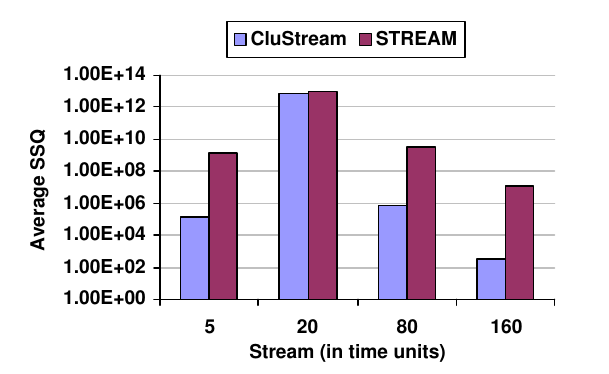
\includegraphics[width=0.9\columnwidth]{./styles/2000h1-orig.png}
%             \caption{SSQ for the original $CluStream$~\cite{clustreamOrig} vs STREAM~\cite{}}\label{fig:2000orig}
%         \end{minipage}
%         \hfill{}
%         \begin{minipage}[r]{1.0\columnwidth}
%             \centering
%             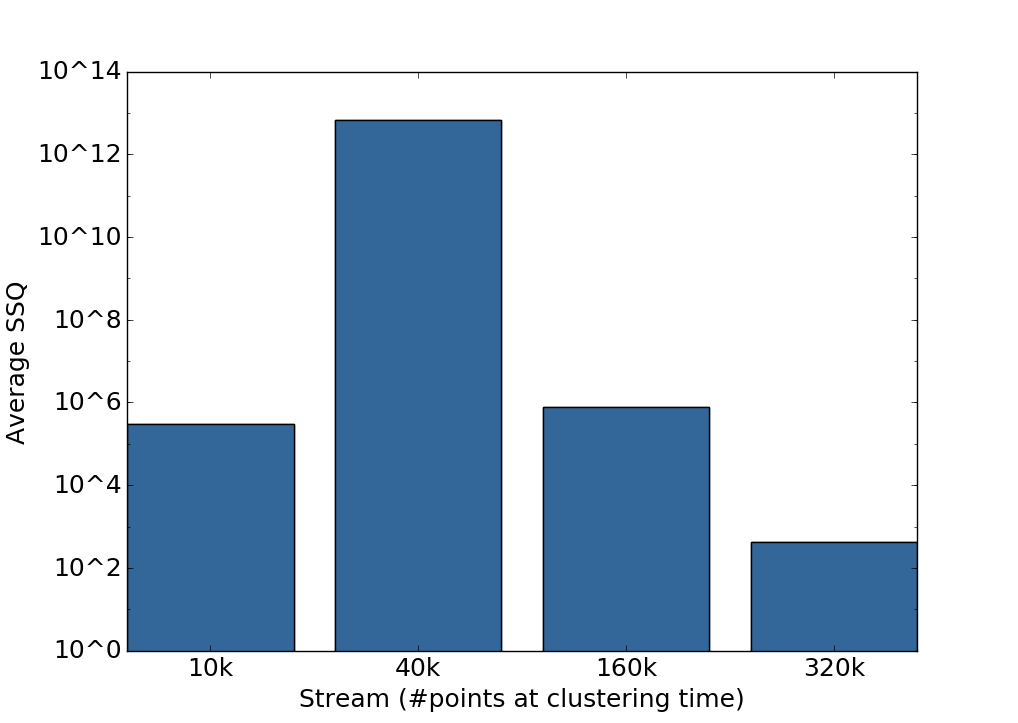
\includegraphics[width=0.9\columnwidth]{./styles/2000h1.png}
%             \caption{SSQ for our $Spark-CluStream$}\label{fig:2000}
%         \end{minipage}
%         \captionsetup{labelformat=empty}
%         \caption{Original $CluStream$ vs SPARK-Clustream.  $DS1$ (Stream speed $v$ = 2,000, $H$=1).}
%         \label{fig:DS1quality}
%     \end{figure*}
    
% Figure \ref{fig:2000orig} shows the results used by the original \textit{CluStream} to show its capabilities against an older method \textit{STREAM}, which is a modified version of K-Means for data streams. The average SSQ for \textit{CluStream} is the most relevant to this test.

% \addtocounter{figure}{-1}
% 
\paragraph{Results for DS2}
% The SSQ for $DS2$ is shown in Figure \ref{fig:DS2quality}.
%  \begin{figure*}[!ht]
%         \begin{minipage}[l]{1.0\columnwidth}
%             \centering
%              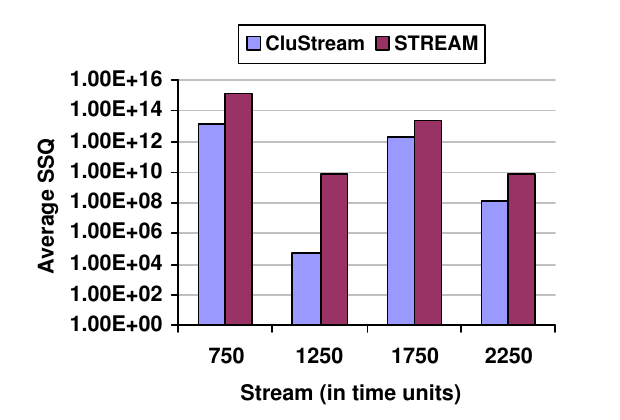
\includegraphics[width=0.9\columnwidth]{./styles/200h256-orig.png}
%             \caption{SSQ for the original $CluStream$~\cite{clustreamOrig} vs STREAM~\cite{}}\label{fig:200h256-orig}
%         \end{minipage}
%         \hfill{}
%         \begin{minipage}[r]{1.0\columnwidth}
%             \centering
%             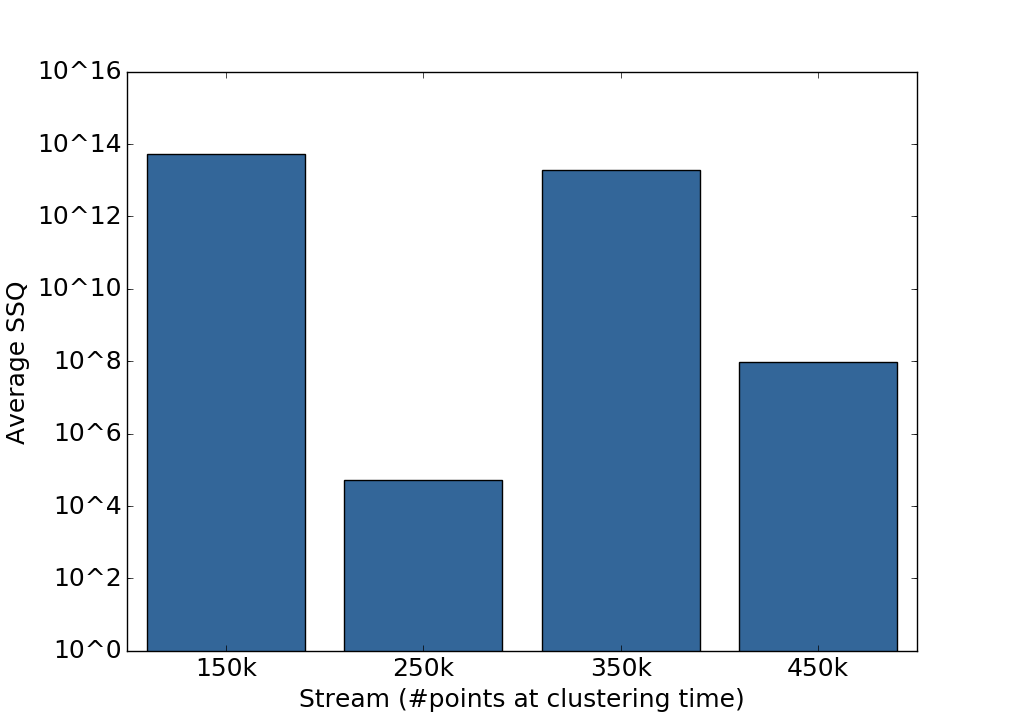
\includegraphics[width=0.9\columnwidth]{./styles/200h256.png}
%             \caption{SSQ for our $Spark-CluStream$}\label{fig:200h256}
%         \end{minipage}
%         \captionsetup{labelformat=empty}
%         \caption{Original $CluStream$ vs SPARK-Clustream. $DS2$ (Stream speed $v$ = 200, $H$=256).}
%         \label{fig:DS2quality}
%     \end{figure*}
%     
%  \addtocounter{figure}{-1}
%  
 
Parameters were set as for $DS1$.
% The measurement is the SSQ again and the same circumstances apply for this case as in the first one with the difference that here $\delta$ and $m$ are relevant. The parameter $m$ is again chosen to be 20: if 200 points are processed every time unit and there are 50 micro-clusters, assuming all 200 points should be distributed uniformly at least every 5 time units leads to $5\frac{200}{50}=20$. An in-depth analysis of the behavior of \textit{CluStream} for different $\delta$'s and $m$'s is out of the scope of this work. 

% Again, the comparison is for the average SSQ. 
The test ran 4 times for \textit{Spark-CluStream} to average the results in both cases, $DS1$ and $DS2$. 
Again, they perform similarly. The exact SSQ scores for $Spark-CluStream$ and the approximated ones from $CluStream$ based on \cite{clustreamOrig} are shown in Table \ref{tab:DS2quality}.

\begin{table*}[t]
\centering
\begin{tabular}{|l|l|l|l|l|}\hline
\textbf{$DS2$ - avg SSQ} & \textbf{150k} & \textbf{250k} & \textbf{350k} & \textbf{450k}\\\hline
CluStream & $10^{13}$-$10^{14}$ & $\approx 10^{5}$ & $10^{12}$-$10^{13}$ & $\approx 10^{8}$\\\hline
Spark-CluStream & $5.402\times10^{13}$ & $5.143\times10^{4}$ & $1.892\times10^{13}$ & $9.646\times10^7$\\\hline
  \end{tabular}
  \caption{$DS2$ - Average SSQ values}
  \label{tab:DS2quality}
\end{table*}

%------------------------------------------------------------------------------------------------------
\subsubsection{$Spark-CluStream$ vs other clustering approaches in SPARK}
\label{sec:expQuality-vs-SPARK}
We compare our \our  against available solutions for stream clustering in Spark and in particular against \textit{Streaming K-Means} and \textit{StreamDM-CluStream}.
% , which is another adaptation of \textit{CluStream} for Spark. 
We report here on their clustering quality, the efficiency issue is discussed in Section~\ref{sec:expScalability}.

We roughly overview these methods hereafter.

% The setup and the dataset are the same as in \ref{validation}, as having already verified results provides the possibility of using those tests to directly compare the results against the other methods. Again, the used measurement is the sum of squares (SSQ).

% Before looking at the results, here are some key considerations for the other methods:

\begin{itemize}
 \item \textit{Streaming K-Means~\footnote{More information: https://databricks.com/blog/2015/01/28/introducing-streaming-k-means-in-spark-1-2.html}}:
 \begin{itemize}
  \item In order to have comparable results, the time horizon $H$ must be interpreted differently. There are two strategies: the first option is to use the parameter \textit{halfLife}, which can be configured to let the algorithm to completely adjust the clusters after $HL$ points or batches.
  \item The alternative would be to set the $decayFactor$, which sets the weight for the clusters of the "old" data (only the current batch is considered "new" data) to calculate the new centroids.
 \end{itemize}
 \item \textit{StreamDM-CluStream~\footnote{More information: http://huawei-noah.github.io/streamDM/}}:
 \begin{itemize}
  \item This adaptation of \textit{CluStream} does not include the offline part as a separate module, meaning that it does not save snapshots and therefore it has to perform the macro-clustering process for every batch. This brings some limitations, the horizon $H$ no longer has the same meaning: the $\delta$ parameter is used instead as an equivalent, relying on the micro-clustering part only and its ability to delete and create new micro-clusters.
\end{itemize}
\end{itemize}

\paragraph{Results on $DS1$}
For the $DS1$ stream the results are shown in Figure~\ref{fig:comparison2000}. The number of clusters $k$ is always 5 for this dataset in all the experiments.
For \textit{Streaming K-Means}, the horizon $H=1$ is transformed to $halfLife=1000$ points. This is because the speed of the stream is 2,000 points per time unit, if the horizon is 1, then only 2000 points are desired to be clustered, and half of that results in 1000 points. 
For the \textit{decayFactor}, it is safe to set it to 0, as that would mean that only the last 2,000 points have influence on the clusters, which is exactly what is desired.
\textit{StreamDM-CluStream} is set up with its default parameters, only changing the horizon to 1 and the number of micro-clusters to 50 in order to match those of \our.

\begin{figure}[h]
 \centering
 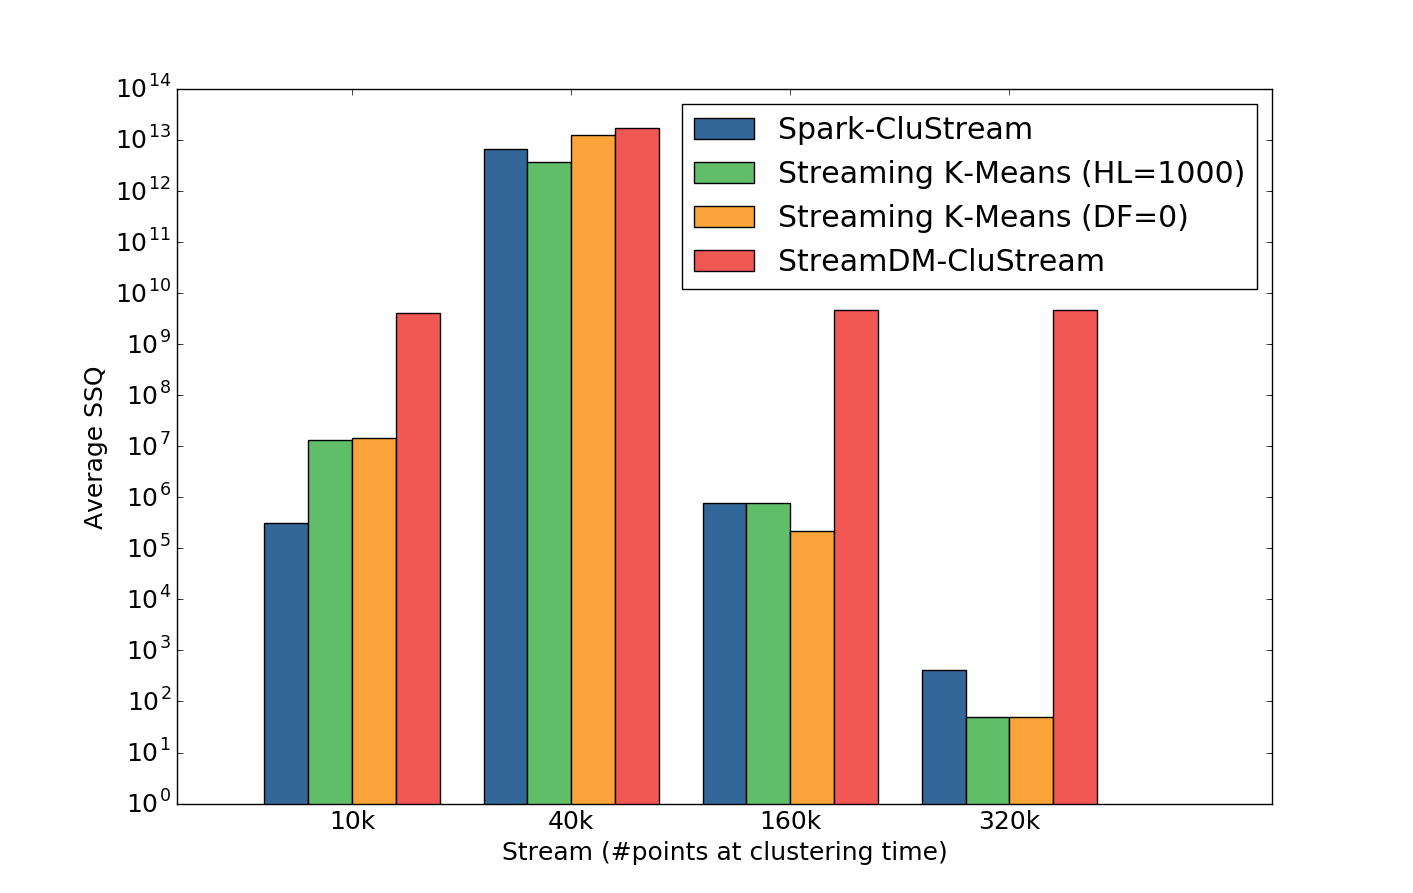
\includegraphics[scale=0.265]{./styles/comparison2000.png}
 \caption{Comparison results: all methods. Stream speed = 2000, H=1}
 \label{fig:comparison2000}
\end{figure}

From Figure~\ref{fig:comparison2000} it can be seen that our \our~delivers results which are very close to those of \textit{Streaming K-Means}. Also, \textit{Streaming K-Means} with the \textit{decayFactor} (DF) is expected to do well on this test as it could be configured to cluster exactly as it was intended for this dataset. 
The surprising results come from \textit{StreamDM-CluStream}, as it performs worse than the rest of the methods, especially for the last two points, i.e.,  at $160k$ and $320k$.
To understand this behavior, we performed another experiment with \our~without snapshots. For both methods we used a horizon $H = 1$ and $m=100$.
\begin{figure}[h]
 \centering
 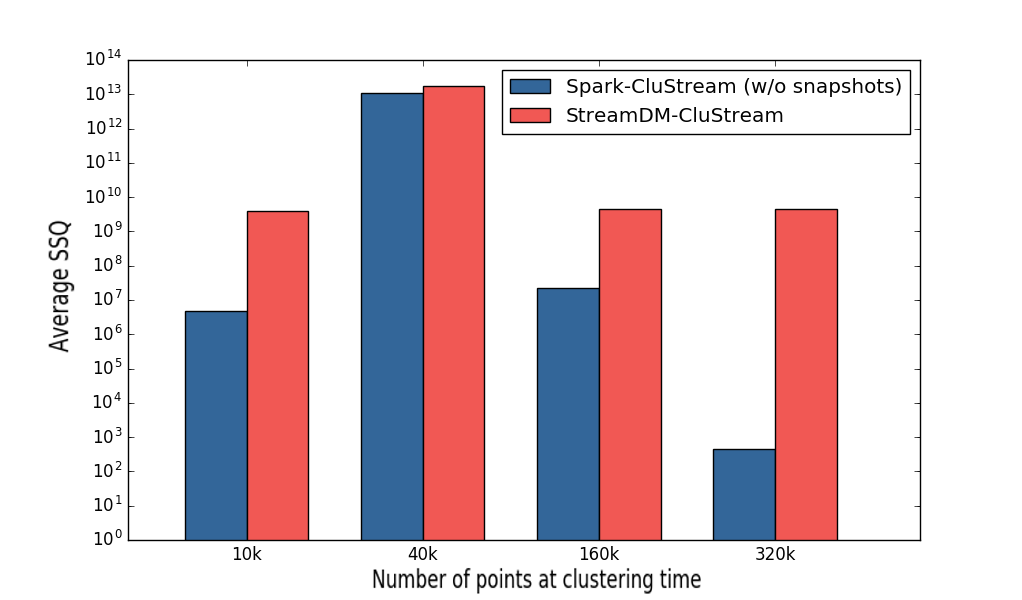
\includegraphics[scale=0.24]{./styles/comparisonNoSnaps.png}
 \caption{\textit{Spark-CluStream} without snapshots. Stream speed=2000, H=1, m=100}
 \label{fig:comparisonNoSnaps}
\end{figure}
From Figure \ref{fig:comparisonNoSnaps} we can see that \our is better comparing to \textit{Spark-CluStream}, even if removing the snapshot part hurts our performance (comparing to the snapshot version).
%  shows poorer results for \textit{Spark-CluStream} in comparison to its original behavior with snapshots, but still delivers noticeably better results than \textit{StreamDM-CluStream}, even though all these tests were executed 4 times and the SSQ erros were averaged to get a better representation of how these methods perform.

%-------------------------------------
\paragraph{Results on $DS2$}
For the $DS2$ stream the results are shown in Figure~\ref{fig:comparison2000}.

Repeating the experiment for the stream with a speed of 200 and a horizon $H=256$ revealed unexpected results. While most parameters for all methods remained the same, for \textit{Streaming K-Means} a new $halfLife$ has to be calculated: multiplying the speed of the stream to the horizon, $200\cdot 256=51200$ shows how many points of the stream are supposed to be clustered at each time, indicating that the parameter should be set to $halfLife=25600$. 


The \textit{decayFactor} strategy at first seems that does not work for such experiment, but considering that the total number of entries is known and exactly the marks at which the clustering process happens, it is possible to calculate an average value to use as a $decayFactor$: 

\begin{itemize}
 \item At 150000 points: $\frac{51200}{150000} \approx 0.3413$, which is the ratio of the points to cluster to the total number of points at that particular time.
 \item At 150000 points: $\frac{51200}{250000} \approx 0.2048$.
 \item At 150000 points: $\frac{51200}{350000} \approx 0.1462$.
 \item At 150000 points: $\frac{51200}{450000} \approx 0.1137$.
\end{itemize}

Averaging those ratios leads to a \textit{decayFactor = 0.2015}, which is a way to determine how important the old data is in comparison to the new one.

\begin{figure}[h!]
 \centering
 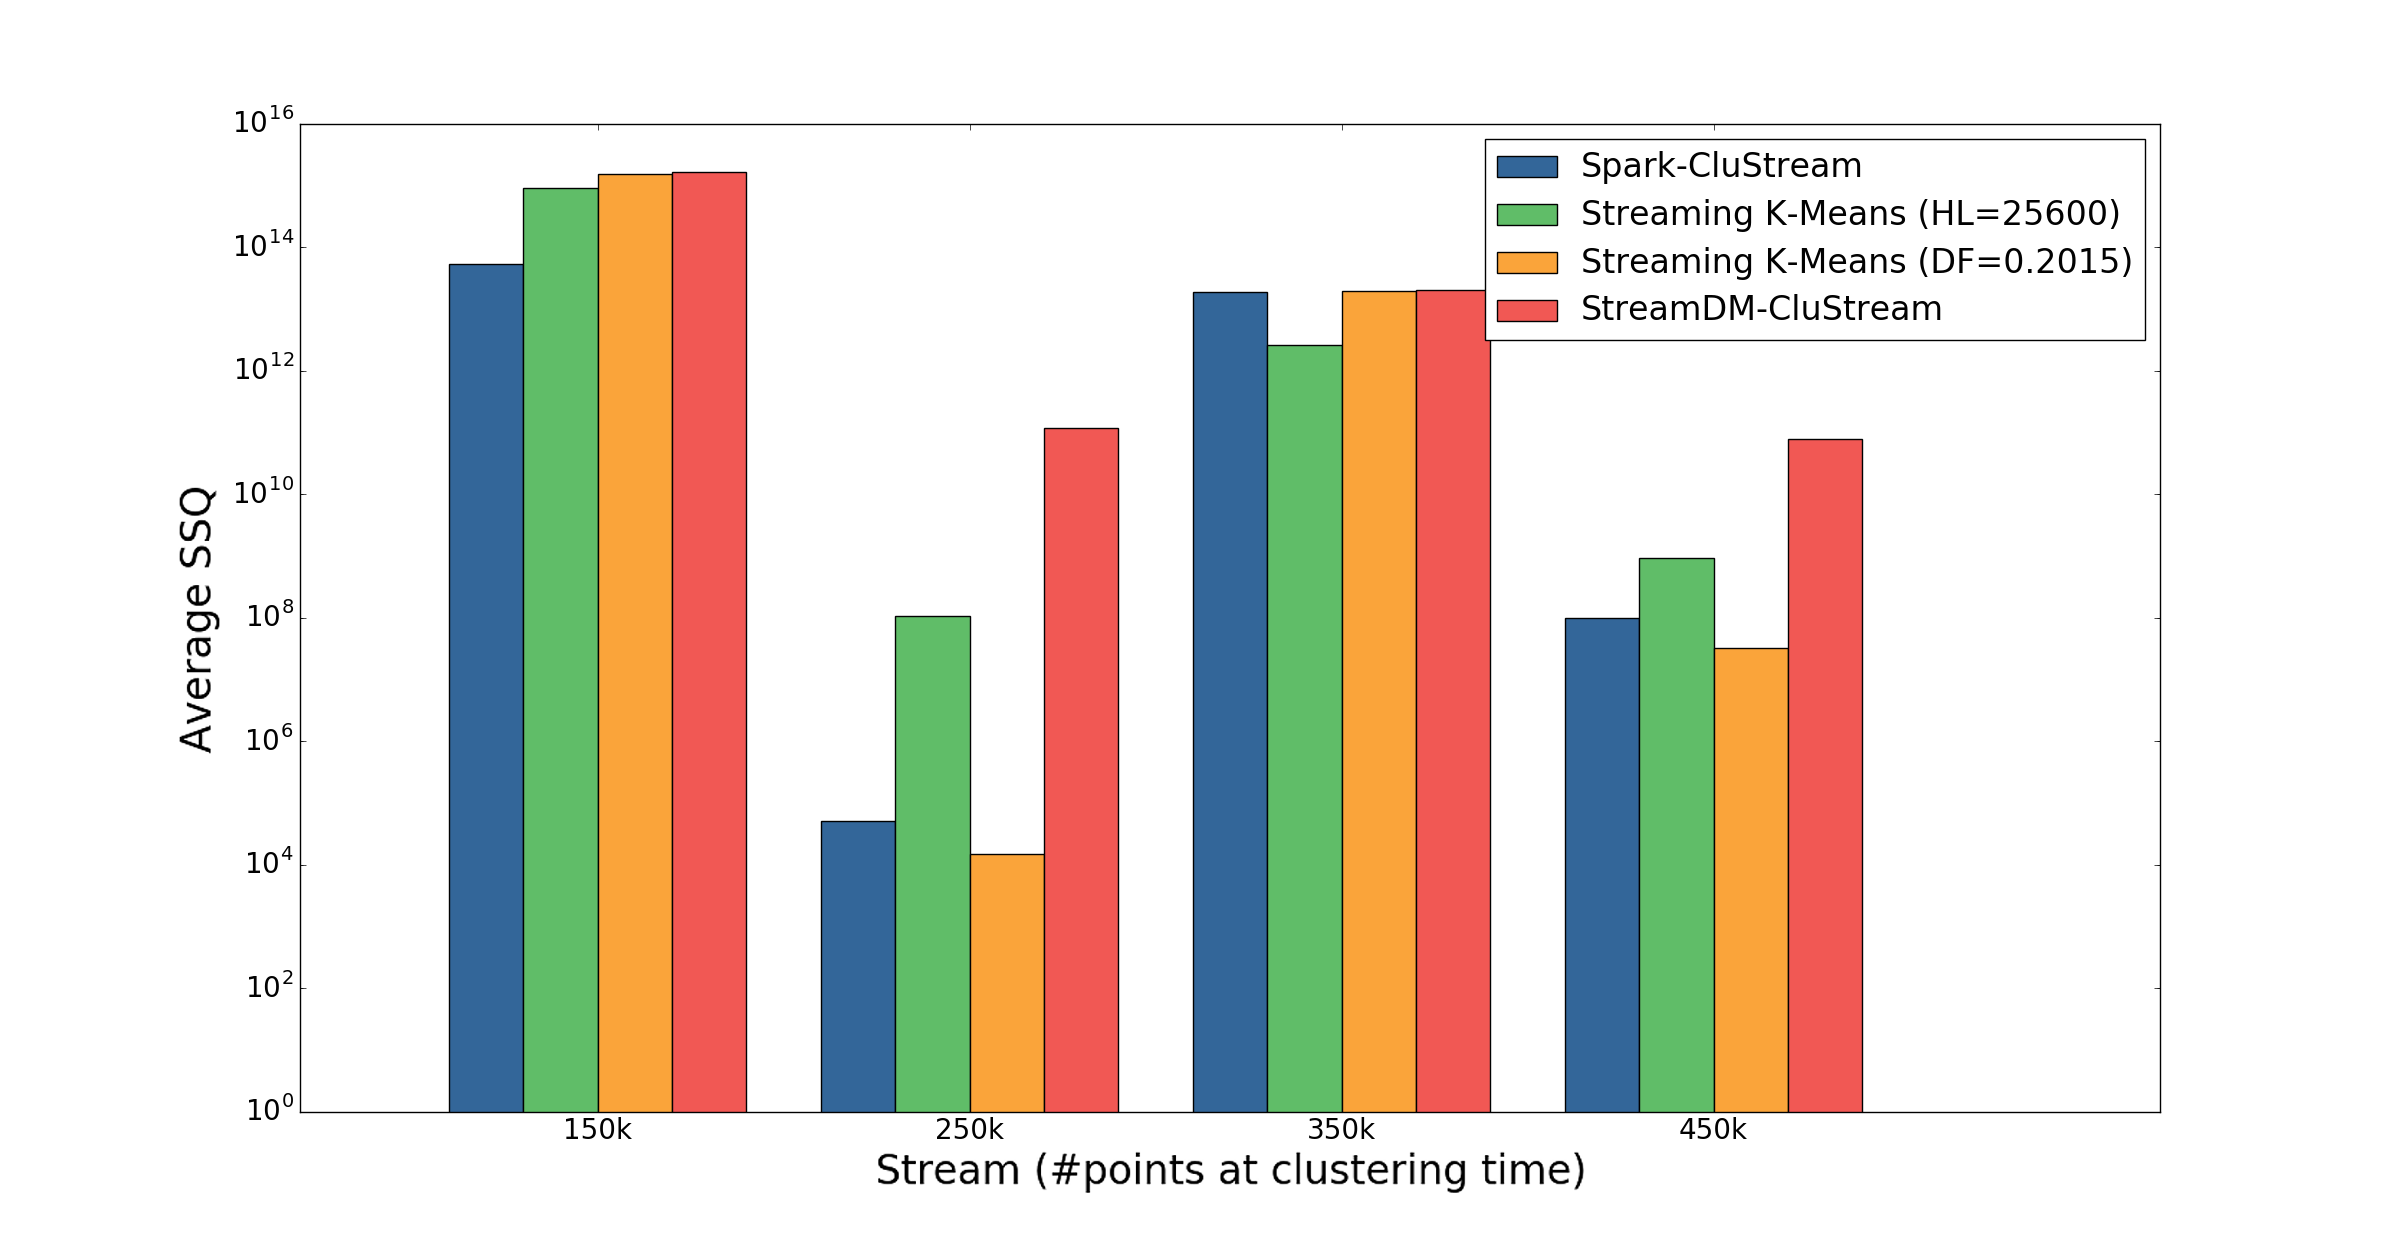
\includegraphics[scale=0.16]{./styles/comparison200.png}
 \caption{Comparison results: all methods. Stream speed = 200, H=256}
 \label{fig:comparison200}
\end{figure}

Figure \ref{fig:comparison200} shows that while \textit{Spark-CluStream} still performs consistently good, \textit{Streaming K-Means} with the \textit{decayFactor} outperformed its relative with the $halfLife$ strategy. Another thing to notice is that \textit{StreamDM-CluStream} still delivered the worse results. 


